\documentclass[lettersize,journal]{IEEEtran}
\usepackage{xeCJK}  %中文；Overleaf 请用 XeLaTeX
\usepackage{amsmath,amsfonts}
\usepackage{algorithmic}
\usepackage{algorithm}
\usepackage{array}
\usepackage[caption=false,font=normalsize,labelfont=sf,textfont=sf]{subfig}
\usepackage{textcomp}
\usepackage{stfloats}
\usepackage{url}
\usepackage{verbatim}
\usepackage{graphicx}
\usepackage{cite}
\usepackage{booktabs}
\usepackage{multirow}
\usepackage{xcolor}
\usepackage{amssymb}
\usepackage[export]{adjustbox}
\usepackage{wrapfig}
\usepackage{subcaption}
\graphicspath{{./images/}}
\hyphenation{op-tical net-works semi-conduc-tor IEEE-Xplore}

% 仍缺实验时的红色占位（定稿前可删除本命令及全部调用）
\newcommand{\ExpTodo}[2]{%
  \textcolor{red}{\textbf{【实验待填-#1】}}%
  \textcolor{red}{（#2）}%
}

\begin{document}

\title{面向边缘部署的红外弱小目标检测可迁移压缩框架}

\author{Guotai Sun, Qin Shu%
\thanks{作者单位、通信作者邮箱等请按最终投稿信息填写。}}

\markboth{IEEE Transactions on Geoscience and Remote Sensing,~Vol.~XX, No.~X, Month~202X}%
{Sun \MakeLowercase{\textit{et al.}}: Transferable Compression for Edge IRSTD}

% 中文双栏草稿阶段关闭 pubid，避免与正文/页脚叠印乱码；英文定稿再恢复
%\IEEEpubid{0000--0000/00\$00.00~\copyright~2021 IEEE}

\maketitle

\begin{abstract}
红外弱小目标检测（Infrared Small-Target Detection, IRSTD）在预警监视、安防与遥感中具有重要应用价值。深度学习方法显著提升了检测精度，但高精度模型参数与计算开销大，难以直接部署到以 Rockchip RK3588 为代表的嵌入式平台。现有轻量化路线或从零设计小网络，或采用通用/任务剪枝，却仍主要依赖权重大小、小波能量等代理指标，且往往缺少\textbf{跨骨干统一协议}与\textbf{板端实测闭环}。
本文提出一套面向红外弱小目标共性、与具体检测骨干解耦的可迁移压缩框架，包含四部分：（1）将任意 IRSTD 分割网络映射为统一剪枝组；（2）融合目标区域加权损失梯度与局部对比先验的小目标敏感性评分，并按尺度分层配额；（3）在共掩码约束下结构化收缩通道宽度并拷贝教师权重；（4）以区域分割损失与输出蒸馏重训恢复性能，再导出 ONNX/RKNN 在板端评估真实资源。
在 DNA-Net、UIU-Net、MSHNet 上的实验表明：学生相对教师参数量下降约 $72\%$--$78\%$、FLOPs 下降约 $54\%$--$62\%$，IoU 总体持平或略升；RK3588 上延迟下降约 $12\%$--$39\%$，同时观察到\textbf{算力下降并不等比转化为墙钟加速}。SCTransNet 上的协议复用实验正在补全。
\end{abstract}

\begin{IEEEkeywords}
红外弱小目标检测，模型压缩，通道剪枝，知识蒸馏，嵌入式部署，可迁移框架，RK3588
\end{IEEEkeywords}

%==============================================================================
\section{引言}
\label{sec:intro}
\IEEEPARstart{S}{ingle}-frame 红外弱小目标检测旨在从单幅红外图像中准确定位尺寸极小、对比度弱、纹理匮乏的目标\cite{DNANet2023,ACM2021}。与可见光通用目标检测不同，目标往往仅占图像极小比例，且易被云层、海杂波与地物纹理淹没，对特征保持与背景抑制提出了极高要求。

近年来，密集嵌套网络 DNA-Net\cite{DNANet2023}、嵌套 U 结构 UIU-Net\cite{UIUNet2023}、多尺度混合网络 MSHNet，以及通道式 Transformer 结构 SCTransNet\cite{SCTransNet2024}等显著提升了公开基准上的交并比（IoU）、检测概率 $P_d$ 与虚警率 $F_a$。然而，精度提升常伴随参数量、浮点运算与访存开销增长，使模型难以部署到算力与功耗受限的边缘平台。工程上，纸面 Params/FLOPs 的下降也并不等价于 NPU 上的真实加速：算子支持、带宽瓶颈与运行时调度都会决定最终可用性。
%\IEEEpubidadjcol % 与 \IEEEpubid 配套；草稿关闭以免叠印

现有高效化研究大致分为两类。一类从零设计轻量网络\cite{RDIAN2023,LWIRSTNet2023,RepISDNet2023,L2SKNet2025}，结构紧凑，部分工作已给出开发板帧率，但容量上限有限，复杂背景上易掉点。另一类对高精度模型做压缩：IRPruneDet\cite{IRPruneDet2024} 将小波结构正则软通道剪枝引入 IRSTD；SAGCP\cite{SAGCP2025} 通过稀疏编码诱导冗余通道删除。二者证明了“IRSTD 需要专用剪枝”，但仍存在不足：（i）重要性多为权重小波能量或稀疏代理，与检测指标的对齐不充分；（ii）跨 CNN/Transformer 的统一压缩协议不完整；（iii）效率评价仍偏 GPU 上的 Params/FLOPs，板端证据不足。

针对上述问题，本文将贡献定位为\textbf{可迁移压缩协议}，而非发布某一改结构的检测器变体。具体而言：
\begin{enumerate}
\item 提出面向 IRSTD 的小目标敏感性评分，融合目标区域加权任务梯度与局部对比先验，并由浅层保护、深层多剪的分层配额导出保留通道。
\item 给出与骨干解耦的剪枝组抽象与共掩码结构化压缩：拓扑（跳连/嵌套/Transformer 层数）保持不变，仅收缩宽度；各骨干仅实现 Adapter。
\item 设计固定的区域分割损失 + 输出知识蒸馏重训配方，将“继承高容量教师判别能力”转化为可检验命题。
\item 以 DNA-Net、UIU-Net、MSHNet（及 SCTransNet）验证协议泛化，并在 RK3588 上闭环评估 Params/FLOPs、RKNN 体积、延迟、进程 RSS 与 NPU 忙碌时间估计。
\end{enumerate}

本文其余部分组织如下：第~\ref{sec:related}~节回顾相关工作；第~\ref{sec:method}~节详述方法（与实现一致）；第~\ref{sec:exp}~节给出实验；第~\ref{sec:concl}~节总结。

%==============================================================================
\section{相关工作}
\label{sec:related}

\subsection{红外弱小目标检测}
传统方法包括滤波、局部对比与低秩稀疏分解等\cite{IPI2013}，可解释性强但对复杂场景鲁棒性有限。深度学习将任务建模为像素级分割：ACM/ALCNet\cite{ACM2021,ALCNet2021}引入上下文与局部对比；DNA-Net\cite{DNANet2023}以密集嵌套交互维持深层小目标响应；UIU-Net\cite{UIUNet2023}采用 U-Net in U-Net；ISNet\cite{ISNet2022}强调形状；SCTransNet\cite{SCTransNet2024}引入空间嵌入的通道式 Transformer。上述高精度模型构成本文压缩的教师起点与泛化验证对象。

\subsection{轻量网络与嵌入式部署}
RDIAN\cite{RDIAN2023}、RepISD-Net\cite{RepISDNet2023}、L$^2$SKNet\cite{L2SKNet2025}、LW-IRSTNet\cite{LWIRSTNet2023}等从结构设计阶段控制复杂度，后者还报告了开发板推理速度。该类工作是“同延迟预算下对照从零轻量模型”的重要基线，但与“从高容量模型压缩并继承能力”的命题不同。

\subsection{模型压缩与 IRSTD 专用剪枝}
通用剪枝如 Network Slimming\cite{NetworkSlimming2017}、Soft Filter Pruning\cite{SoftFilterPruning2018}等面向分类，易误伤 IRSTD 所需的浅层空间细节。IRPruneDet\cite{IRPruneDet2024}、SAGCP\cite{SAGCP2025} 证明了任务专用剪枝的必要性。知识蒸馏\cite{HintonDistill2015}为剪后恢复提供了通用工具。本文与之差异在于：面向小目标的区域敏感评分、跨架构共掩码协议、蒸馏恢复与\textbf{板端效率闭环}一体。

%==============================================================================
\section{方法}
\label{sec:method}

\subsection{问题形式化}
\label{sec:problem}
给定已训练的 IRSTD 分割教师网络 $M_T$、精度容差 $\varepsilon$ 与复杂度/延迟预算 $B$，目标是得到学生网络 $M_S$，使得
\begin{equation}
\label{eq:obj}
\mathrm{Acc}(M_S)\ge \mathrm{Acc}(M_T)-\varepsilon,\qquad
\mathrm{Cost}(M_S)\le B,
\end{equation}
其中 $\mathrm{Acc}$ 采用 IoU（及 $P_d$、$F_a$），$\mathrm{Cost}$ 可为 Params、FLOPs 与板端延迟。关键约束是：压缩协议应尽量与 $M_T$ 的具体拓扑解耦。

\subsection{总体框架}
\label{sec:overview}
如图~\ref{fig:pipeline}所示，框架包含四步：
\textbf{Adapter 枚举剪枝组} $\rightarrow$
\textbf{小目标敏感性评分} $\rightarrow$
\textbf{结构化压缩与权重拷贝} $\rightarrow$
\textbf{蒸馏重训与板端部署}。

\begin{figure*}[!t]
\centering
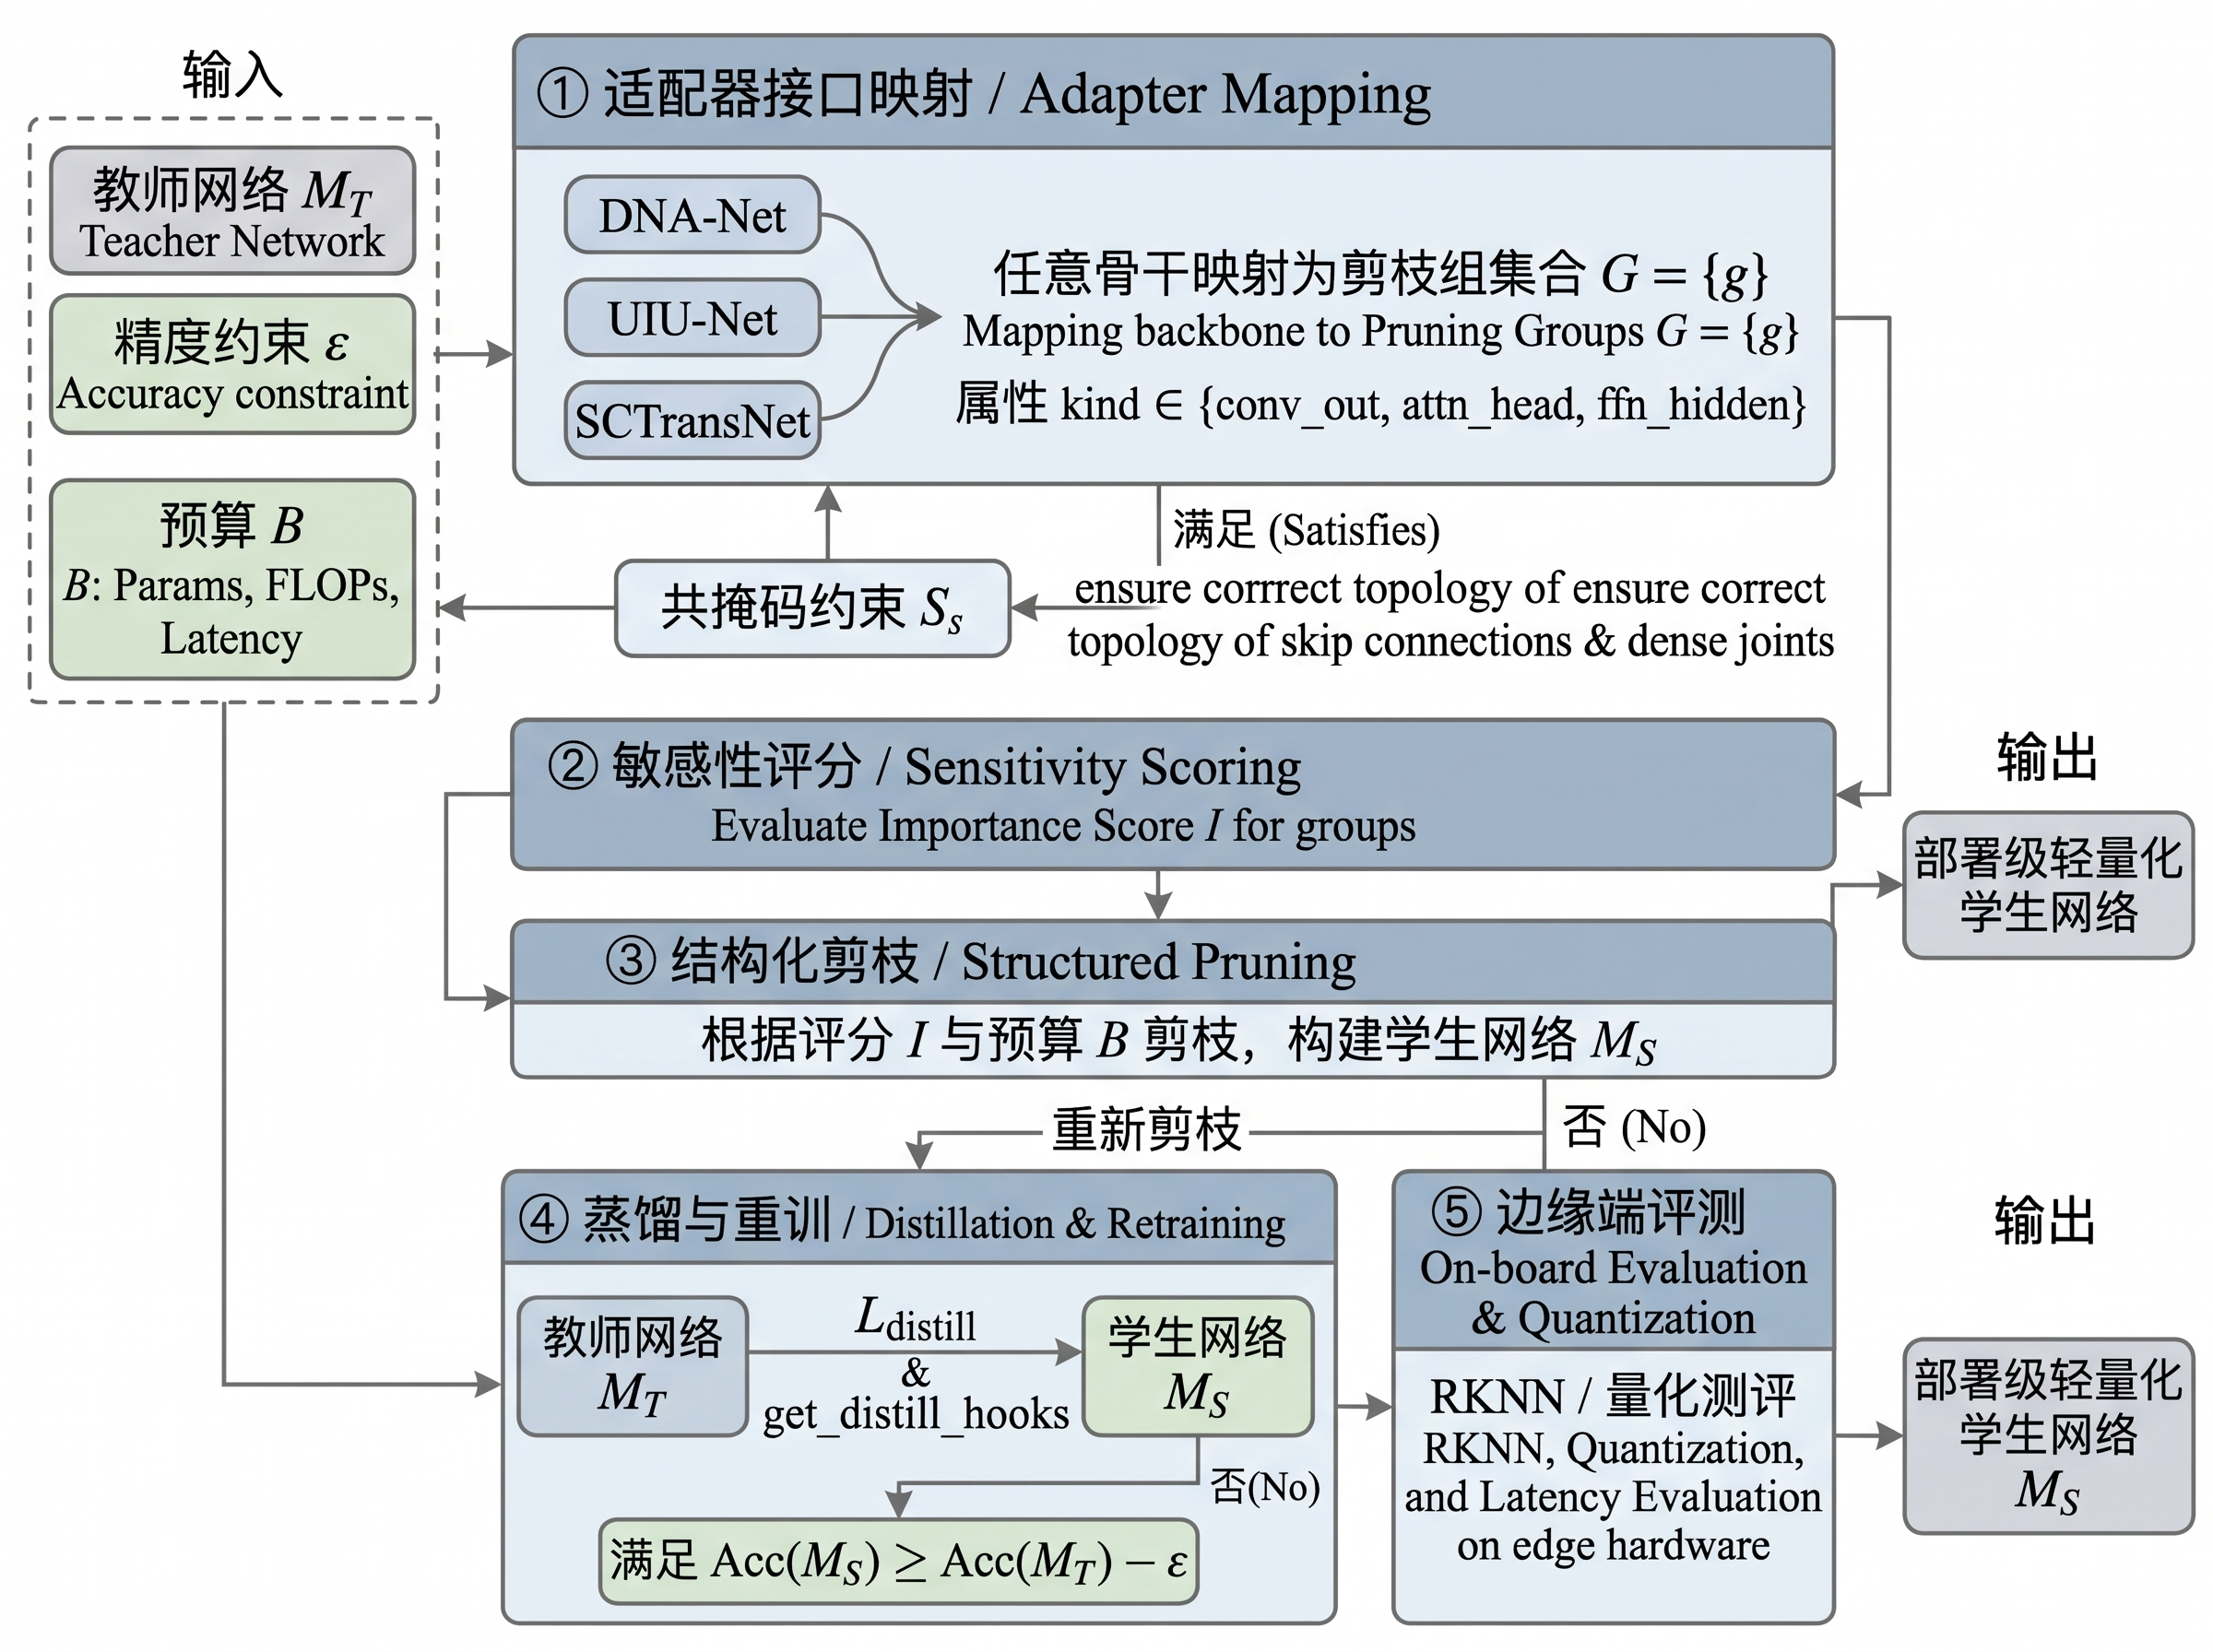
\includegraphics[width=0.92\textwidth]{fig1.png}
\caption{所提可迁移压缩框架总体流程：Adapter 映射、敏感性评分、共掩码结构化变窄、蒸馏恢复与 RK3588 部署评估。}
\label{fig:pipeline}
\end{figure*}

\subsection{剪枝组抽象与模型适配}
\label{sec:adapter}
为屏蔽结构差异，将任意骨干映射为剪枝组集合 $\mathcal{G}=\{g\}$。每个组包含：类型（本文实现以 $\mathrm{conv\_out}$ 为主）、阶段编号 $\mathrm{stage\_id}$、可剪通道数 $C_g$，以及需同步切片的模块集合。

\textbf{共掩码约束：}对存在跳跃连接或密集拼接的尺度 $s$，所有输出宽度同为该尺度通道维的组共享同一保留下标集合 $S_s$。该约束保证 DNA-Net 嵌套节点、UIU-Net/MSHNet 跳连、SCTransNet 编解码拼接在变窄后仍拓扑合法。

每个骨干仅实现适配器：\texttt{enumerate\_groups}、\texttt{build\_student}（含权重切片）、以及用于评分的特征/梯度钩子。评分、配额、蒸馏与导出主体不随模型复制。各骨干实例化见表~\ref{tab:adapter}。

\begin{table}[!t]
\caption{骨干 Adapter 实例化（与实现一致）}
\label{tab:adapter}
\centering
\begin{tabular}{|p{2.0cm}|p{5.6cm}|}
\hline
骨干 & 剪枝组要点 \\
\hline
DNA-Net & 5 档 \texttt{nb\_filter}；尺度共掩码；Res-CBAM 同步切片 \\
\hline
MSHNet & 5 档 \texttt{param\_channels}；Res+CBAM 同步切片 \\
\hline
UIU-Net & 4 档 stage 宽度；RSU 拓扑不变；mid 通道按比例缩放 \\
\hline
SCTransNet & 4 档 CNN 宽度；\texttt{KV\_size}$=\sum$ 通道；Transformer \textbf{层数/头数不变} \\
\hline
\end{tabular}
\end{table}

\subsection{小目标敏感性评分}
\label{sec:importance}
对组 $g$ 的第 $c$ 个输出通道，定义
\begin{equation}
\label{eq:I}
I(g,c)=\alpha\,\hat{I}_{\mathrm{task}}(g,c)+(1-\alpha)\,\hat{I}_{\mathrm{contrast}}(g,c),
\end{equation}
其中 $\hat{\cdot}$ 表示组内 min-max 归一化，默认 $\alpha=0.7$。

\textbf{任务项 $I_{\mathrm{task}}$：}
采用目标区域加权 SoftIoU：在真值 mask 的膨胀邻域内计算损失并对教师反传，取残差块末层卷积（如 \texttt{conv2}）权重梯度幅值，按输出通道聚合，再在若干训练 batch 上平均。相对全局损失，该设计减轻背景像素对重要性估计的主导。

\textbf{对比项 $I_{\mathrm{contrast}}$：}
记组输出特征为 $A$，则
\begin{equation}
\label{eq:contrast}
I_{\mathrm{contrast}}(g,c)=\mathbb{E}\!\big[\bar{A}_{c}^{\mathrm{tgt}}-\bar{A}_{c}^{\mathrm{bg}}\big],
\end{equation}
即目标邻域平均响应与背景平均响应之差，体现红外局部对比先验。

\textbf{分层配额：}
按 $\mathrm{stage\_id}$ 设定剪枝率 $p_s$（浅层小、深层大）。例如五尺度网络默认
$p=(0.2,0.3,0.4,0.5,0.6)$，四尺度为 $(0.2,0.3,0.4,0.5)$。组内按 $I$ 降序保留约 $(1-p_s)C_g$ 个通道（SCTransNet 另强制偶数通道以兼容分组卷积）。
为避免在庞大搜索空间中进行耗时的硬件在环搜索，本文将式~\eqref{eq:obj} 中的预算约束 $B$ 实例化为一组经验预设的分层收缩配额 $\{p_s\}$（浅层保护、深层激进），通过单次确定性压缩即可实现约 $55\%$--$60\%$ 的 FLOPs 削减；若目标板端延迟等具体 $B$ 已知，可在该配额邻域内做轻量网格搜索或二分校准，而不改变协议主体。

\textbf{可选校准（投稿增强）：}
对 Top-$k$/Bottom-$k$ 通道敲除并绘制 IoU 掉点曲线，可与 $\ell_1$、随机剪枝对照，以加强 $I$ 的因果解释。
\ExpTodo{Ex08}{补敲除校准曲线；当前主文以分层配额+跨骨干复现为主证据。}

\subsection{结构化压缩}
\label{sec:prune}
在配额 $\{p_s\}$ 下得到保留集合 $\{S_s\}$，重建更窄学生 $M_S$，并将教师卷积/BN（及注意力中与通道绑定的参数）按索引切片拷贝。硬约束包括：同 stage 共掩码；BN 统计量同步；分割头输出维不剪。过程\textbf{不修改}跳连/嵌套/Transformer 层数语义，仅改变宽度。

\subsection{蒸馏重训与板端部署}
\label{sec:distill}
剪后优化目标（与实现一致）为
\begin{equation}
\label{eq:loss}
\begin{aligned}
\mathcal{L}=&\ 
\lambda_{\mathrm{seg}}\,\mathcal{L}_{\mathrm{seg}}(M_S,y)
+\lambda_{\mathrm{region}}\,\mathcal{L}_{\mathrm{region}}(M_S,y)\\
&+\lambda_{\mathrm{kd}}\,\mathcal{L}_{\mathrm{KD}}\!\big(M_S(x),M_T(x)\big),
\end{aligned}
\end{equation}
其中 $\mathcal{L}_{\mathrm{seg}}$ 为各骨干习惯的分割损失（SoftIoU/BCE 及多尺度头），$\mathcal{L}_{\mathrm{region}}$ 为目标区域加权 SoftIoU，$M_T$ 冻结；$\mathcal{L}_{\mathrm{KD}}$ 为输出掩膜的 MSE（logits 经 sigmoid 或教师已输出概率）。默认 $\lambda_{\mathrm{seg}}=\lambda_{\mathrm{kd}}=1$，$\lambda_{\mathrm{region}}=0.5$，蒸馏约 $200$ epoch。

板端阶段导出固定分辨率 ONNX，使用 rknn-toolkit2 转为 RKNN，在 RK3588 上测量延迟、进程 RSS、NPU 负载并估计忙碌时间 $\approx\mathrm{latency}\times\mathrm{mean(NPU\%)}$。评分决定“剪谁”，板端决定“是否真快”，二者解耦。

\begin{algorithm}[!t]
\caption{可迁移 IRSTD 压缩协议}
\label{alg:main}
\begin{algorithmic}
\STATE \textbf{输入：}教师 $M_T$，数据 $\mathcal{D}$，预算 $B$ 的实例化配额 $\{p_s\}$，蒸馏轮数 $E$
\STATE $\mathcal{G}\leftarrow \texttt{Adapter.enumerate\_groups}(M_T)$
\STATE 在 $\mathcal{D}$ 上计算 $I(g,c)$（式~\eqref{eq:I}）；按 $\{p_s\}$ 生成 $\{S_s\}$
\STATE $M_S\leftarrow \texttt{Adapter.build\_student}(M_T,\{S_s\})$；切片拷贝权重
\STATE 按式~\eqref{eq:loss} 蒸馏 $E$ 轮，保存验证集最佳学生
\STATE 导出 ONNX/RKNN；板端测评
\STATE \textbf{输出：}$M_S$
\end{algorithmic}
\end{algorithm}

%==============================================================================
\section{实验}
\label{sec:exp}

\subsection{实验设置}
\label{sec:setup}

\subsubsection{数据集与协议}
采用 NUAA-SIRST、NUDT-SIRST、IRSTD-1k 与 SIRST-V2。数据按各数据集官方或社区常用的 \texttt{trainval.txt}/\texttt{test.txt} 划分；训练输入分辨率以各教师默认为主。DNA-Net/MSHNet/SCTransNet 常用 $256\times256$。UIU-Net 与官方设定一致：教师与学生蒸馏均采用 rescale $320$、随机 crop $288$；表~\ref{tab:main_iou} 中 UIU 的 IoU 亦在同一评测管线（测试 rescale $320$、无 crop）下统计。为保证跨骨干横向可比，表~\ref{tab:resource} 的 RK3588 资源对比统一在固定输入 $256\times256$ 下测量，该设定仅用于板端效率，不改变精度表的分辨率协议。

\subsubsection{评价指标}
精度：IoU（主指标）；目标级 $P_d$、$F_a$ 作为补充。
\ExpTodo{Ex05b}{补齐各骨干学生完整 $P_d$/$F_a$ 列（与教师同评测脚本）。}
效率：Params(M)、FLOPs(G，$\approx 2\times$MACs)、RKNN 体积(MB)；板端：延迟 mean(ms)、进程 RSS mean、估计 NPU 忙碌 ms/帧（非功率计）。

\subsubsection{实现细节}
PyTorch 训练；敏感性评分默认 $50$ batch，$\alpha=0.7$，膨胀核半径 $3$。蒸馏默认 $200$ epoch；DNA-Net/MSHNet 优化器与教师一致（常用 Adagrad），UIU-Net/SCTransNet 常用 Adam。板端：RK3588，librknnrt $2.5.0$，\texttt{core\_mask}$=7$，warmup $20$、iters $80$，输入 $1\times256\times256\times3$（SCTrans 灰度输入按实现为单通道）。随机种子固定为 $42$。

\subsubsection{对比与定位}
本文主对比为\textbf{同骨干教师 vs 学生}（验证压缩有效且可迁移），并报告跨 DNA-Net/UIU-Net/MSHNet 的板端资源表。
\ExpTodo{Ex04}{补充与 IRPruneDet/SAGCP/从零轻量网络在相近 Params 或板端延迟下的对照（H1）。}

\subsection{主结果：精度}
\label{sec:main_results}

表~\ref{tab:main_iou}给出教师/学生 best IoU。总体结论：\textbf{压缩后 IoU 未系统性下降}；UIU-Net 与 MSHNet 上师生基本持平（均值差约 $0.02\%$--$0.15\%$），个别数据集略降（如 MSHNet 在 IRSTD-1k/SIRST-V2）。
DNA-Net 上学生均值由 $0.7250$ 升至 $0.7696$，涨幅明显高于其余骨干。对此我们作如下解释，而非仅归因于“蒸馏偶然增益”：（1）DNA-Net 原生五层密集嵌套在 NUAA/NUDT 等小样本红外集上存在明显过参数化与过拟合，结构化变窄相当于强结构正则，有助于泛化；（2）学生重训配方额外使用了局部区域加权损失 $\mathcal{L}_{\mathrm{region}}$，强化边界与小目标收敛，而教师日志中的 IoU 对应其原始训练目标。该解释可由后续表~\ref{tab:distill} 的蒸馏恢复消融（仅 GT / 分割+区域 / 完整配方）加以佐证；同时，为排除“教师未训充分”的质疑，定稿前建议用与学生相同的评测脚本对教师权重做一次复测并报告 epoch/早停设置。

\begin{table}[!t]
\caption{教师 vs 学生 best IoU（四数据集）。SCTransNet 学生结果待训练完成后填入。}
\label{tab:main_iou}
\centering
\footnotesize
\begin{tabular}{|l|c|c|c|c|c|}
\hline
方法 & NUAA & NUDT & IRSTD-1k & SIRST-V2 & 均值 \\
\hline
DNA-Net 教师 & 0.7171 & 0.8488 & 0.6230 & 0.7112 & 0.7250 \\
本文-DNA 学生 & 0.7387 & 0.9226 & 0.6706 & 0.7464 & 0.7696 \\
\hline
UIU-Net 教师 & 0.7686 & 0.8596 & 0.6376 & 0.8558 & 0.7804 \\
本文-UIU 学生 & 0.7741 & 0.8471 & 0.6439 & 0.8625 & 0.7819 \\
\hline
MSHNet 教师 & 0.6909 & 0.7558 & 0.6779 & 0.7320 & 0.7142 \\
本文-MSH 学生 & 0.6959 & 0.7729 & 0.6653 & 0.7220 & 0.7140 \\
\hline
SCTrans 教师 & -- & -- & -- & -- & -- \\
本文-SCTrans 学生 & -- & -- & -- & -- & -- \\
\hline
\end{tabular}
\end{table}

\ExpTodo{Ex05}{填入 SCTransNet 教师/学生 IoU；必要时统一复测脚本复核 DNA/UIU/MSH 的 $P_d$/$F_a$。}

\begin{figure}[!t]
\centering
\fbox{\parbox{0.88\columnwidth}{\centering\vspace{0.7cm}
\textbf{【图位 Fig.2｜实验待填-Ex06】}\\
IoU--Params / IoU--FLOPs Pareto（教师点与学生点连线）
\vspace{0.7cm}}}
\caption{精度--复杂度 Pareto 示意（待绘图）。}
\label{fig:pareto}
\end{figure}

\subsection{复杂度与板端资源（NUAA，$256$）}
\label{sec:edge}

表~\ref{tab:resource}汇总三套已完成板端闭环的骨干。可以观察到稳定模式：
\begin{itemize}
\item Params 降约 $72\%$--$78\%$，FLOPs 降约 $54\%$--$62\%$，RKNN 体积显著下降；
\item 墙钟延迟有收益，但\textbf{降幅通常小于 FLOPs 降幅}（DNA-Net 尤为明显）；
\item 估计 NPU 忙碌时间在 DNA-Net/MSHNet 上近似持平，UIU-Net 上下降更明显。
\end{itemize}

\begin{table*}[!t]
\caption{NUAA-SIRST、$256\times256$、RK3588 资源对比（教师 $\rightarrow$ 学生）。延迟/RSS 为 \texttt{resource\_bench}，$80$ iters。}
\label{tab:resource}
\centering
\footnotesize
\begin{tabular}{|l|c|c|c|c|c|c|}
\hline
骨干 & Params (M) & FLOPs (G) & RKNN (MB) & 延迟 mean (ms) & RSS mean (MB) & NPU busy (ms/帧) \\
\hline
DNA-Net & $4.69\!\rightarrow\!1.13$ & $27.85\!\rightarrow\!12.92$ & $14.6\!\rightarrow\!8.0$ & $1034\!\rightarrow\!913$ & $90.7\!\rightarrow\!80.5$ & $249\!\rightarrow\!256$ \\
 & (\textbf{$-75.8\%$}) & (\textbf{$-53.6\%$}) & ($-45\%$) & (\textbf{$-11.7\%$}) & ($-11.2\%$) & ($\approx$持平) \\
\hline
UIU-Net & $50.54\!\rightarrow\!13.89$ & $109.0\!\rightarrow\!46.8$ & $113.8\!\rightarrow\!34.7$ & $658.9\!\rightarrow\!404.3$ & $198.0\!\rightarrow\!110.8$ & $309\!\rightarrow\!221$ \\
 & (\textbf{$-72.5\%$}) & (\textbf{$-57.1\%$}) & (\textbf{$-69.5\%$}) & (\textbf{$-38.6\%$}) & (\textbf{$-44.1\%$}) & (\textbf{$-28.3\%$}) \\
\hline
MSHNet & $4.07\!\rightarrow\!0.89$ & $12.22\!\rightarrow\!4.70$ & $10.58\!\rightarrow\!4.43$ & $478.9\!\rightarrow\!374.2$ & $59.6\!\rightarrow\!53.0$ & $105\!\rightarrow\!100$ \\
 & (\textbf{$-78.2\%$}) & (\textbf{$-61.5\%$}) & (\textbf{$-58.1\%$}) & (\textbf{$-21.9\%$}) & ($-11.1\%$) & ($\approx$持平) \\
\hline
SCTransNet & -- & -- & -- & -- & -- & -- \\
\hline
\end{tabular}
\end{table*}

\ExpTodo{Ex13}{SCTransNet 导出 RKNN 后补表~\ref{tab:resource}最后一行；可选补充 INT8 与功耗计数据。}

\subsection{消融与机制验证（投稿强化项）}
\label{sec:ablation}

为保证 TGRS 审稿所需的机制证据，建议在 DNA-Net（第一试验床）上补齐下列对照；当前主文已具备跨骨干复现与板端闭环，消融表仍为增强项。

\begin{table}[!t]
\caption{重要性准则对照（相同压缩率，DNA-Net/NUAA）。\textcolor{red}{待填}}
\label{tab:criterion}
\centering
\begin{tabular}{|l|c|c|c|}
\hline
准则 & $\mathrm{IoU}\uparrow$ & $\mathrm{P}_d\uparrow$ & $\mathrm{F}_a\downarrow$ \\
\hline
随机剪枝 & -- & -- & -- \\
\hline
$\ell_1$ 权重 & -- & -- & -- \\
\hline
仅 $I_{\mathrm{task}}$ & -- & -- & -- \\
\hline
仅 $I_{\mathrm{contrast}}$ & -- & -- & -- \\
\hline
本文 $I$（完整） & -- & -- & -- \\
\hline
\end{tabular}
\end{table}

\begin{table}[!t]
\caption{蒸馏恢复消融（DNA-Net/NUAA）。\textcolor{red}{待填}}
\label{tab:distill}
\centering
\begin{tabular}{|l|c|}
\hline
设置 & IoU \\
\hline
剪后不重训 & -- \\
\hline
仅 GT 分割损失 & -- \\
\hline
分割 + 区域损失 & -- \\
\hline
分割 + 区域 + 输出 KD（本文） & -- \\
\hline
\end{tabular}
\end{table}

\ExpTodo{Ex07}{填表~\ref{tab:criterion}。}
\ExpTodo{Ex10}{填表~\ref{tab:distill}。}
\ExpTodo{Ex09}{$\alpha$ 与分层配额敏感性曲线。}

\subsection{定性结果}
\label{sec:qual}

\begin{figure*}[!t]
\centering
\fbox{\parbox{0.92\textwidth}{\centering\vspace{0.9cm}
\textbf{【图位 Fig.4｜实验待填-Ex15】}\\
原图 / GT / 教师 / 学生；标注正确检测、漏检与虚警。
\vspace{0.9cm}}}
\caption{定性检测结果对比。}
\label{fig:qual}
\end{figure*}

\subsection{讨论}
\label{sec:discuss}
\textbf{有效性：}跨 DNA-Net/UIU-Net/MSHNet，压缩在保持 IoU 的同时显著降低 Params/FLOPs，并在 RK3588 上获得可测的延迟与内存收益，说明协议可迁移且面向部署可用。

\textbf{FLOPs--延迟鸿沟：}DNA-Net 上 FLOPs 降约一半而延迟仅降约 $12\%$，提示 NPU 推理受算子形态、带宽与调度影响；论文应将其作为边缘 AI 的必要讨论，而非只报告 FLOPs。

\textbf{局限：}（1）当前 SCTransNet 仅压缩 CNN 宽度，未削减 Transformer 层数；（2）敲除校准与外部剪枝基线仍待补全；（3）单位帧能耗需功率计；（4）极低 SCR 场景下的失败案例需定性展示。
\ExpTodo{Ex16}{补充失败案例可视化与量化敏感讨论。}

%==============================================================================
\section{结论}
\label{sec:concl}
本文面向嵌入式红外弱小目标检测，提出与骨干解耦的可迁移压缩框架：以小目标敏感性评分为核心识别冗余通道，在共掩码约束下结构化变窄，经区域损失与输出蒸馏恢复后，在 RK3588 上验证真实效率。实验表明，DNA-Net/UIU-Net/MSHNet 学生相对教师可实现约 $72\%$--$78\%$ 的参数压缩与约 $54\%$--$62\%$ 的 FLOPs 下降，同时 IoU 总体保持；板端延迟下降约 $12\%$--$39\%$，并揭示算力指标与墙钟加速的不等价性。

未来工作包括：补全 SCTransNet 板端闭环与准则/蒸馏消融、量化感知压缩、视频序列扩展，以及更广泛芯片平台验证。

%==============================================================================
\section*{Acknowledgments}
\ExpTodo{Ex18}{基金号与致谢对象待填。}

%==============================================================================
\appendix
\section*{仍缺实验清单（内部；投稿前删除）}
\begin{center}
\footnotesize
\begin{tabular}{|c|l|p{6.2cm}|}
\hline
编号 & 优先级 & 内容 \\
\hline
P0 & 必须 & SCTransNet 学生 IoU + RK3588 资源行 \\
\hline
P0 & 必须 & 统一脚本补 $P_d$/$F_a$ \\
\hline
P1 & 强烈建议 & 表~\ref{tab:criterion}/\ref{tab:distill} 消融（DNA-Net） \\
\hline
P1 & 强烈建议 & Fig.~\ref{fig:pareto}/\ref{fig:qual} \\
\hline
P2 & 增强 & 敲除曲线；与 IRPruneDet/SAGCP/轻量网络同预算对照 \\
\hline
P2 & 增强 & INT8 掉点、功耗计 \\
\hline
\end{tabular}
\end{center}

\noindent\textbf{与旧稿差异说明（写作对齐实现）：}
方法损失以式~\eqref{eq:loss}为准（未将特征蒸馏作为默认项）；SCTransNet Adapter 以 CNN 通道+KV 联动为主，而非默认剪注意力头；MSHNet 已纳入主实验。

%==============================================================================
\bibliographystyle{IEEEtran}
\bibliography{refs}

\vspace{11pt}

\begin{IEEEbiographynophoto}{Guotai Sun}
作者简介待填。
\end{IEEEbiographynophoto}

\begin{IEEEbiographynophoto}{Qin Shu}
作者简介待填。
\end{IEEEbiographynophoto}

\vfill

\end{document}
